\documentclass[14pt]{extreport}
\usepackage{cmap}
\usepackage[utf8]{inputenc}
\usepackage[english,ukrainian]{babel}
\usepackage{graphicx}
\usepackage{geometry}
\usepackage{listings}
\usepackage{amsmath}
\usepackage{float}
\geometry{
	a4paper,
	left=20mm,
	right=20mm,
	top=20mm,
	bottom=20mm
}
\lstset{
	language=bash,
	tabsize=4,
	breaklines,
	keepspaces,
	showstringspaces=false,
}
\graphicspath{ {./pictures} }
\setlength{\parindent}{4em}

\newcommand\subject{Кросплатформне програмування}
\newcommand\lecturer{доцент кафедри ПЗ\\Дяконюк Л.М.}
\newcommand\teacher{ст. викл. кафедри ПЗ\\Шкраб Р.Р.}
\newcommand\mygroup{ПЗ-32}
\newcommand\lab{3}
\newcommand\theme{Робота з колекціями}
\newcommand\purpose{Навчитися працювати з колекціями}

\begin{document}
\begin{normalsize}
	\begin{titlepage}
		\thispagestyle{empty}
		\begin{center}
			\textbf{МІНІСТЕРСТВО ОСВІТИ І НАУКИ УКРАЇНИ\\
				НАЦІОНАЛЬНИЙ УНІВЕРСИТЕТ "ЛЬВІВСЬКА ПОЛІТЕХНІКА"}
		\end{center}
		\begin{flushright}
			Інститут \textbf{КНІТ}\\
			Кафедра \textbf{ПЗ}
		\end{flushright}
		\vspace{160pt}
		\begin{center}
			\textbf{ЗВІТ}\\
			\vspace{10pt}
			До лабораторної роботи № \lab\\
			\textbf{На тему}: “\textit{\theme}”\\
			\textbf{З дисципліни}: “\subject”
		\end{center}
		\vspace{40pt}
		\begin{flushright}
			
			\textbf{Лектор}:\\
			\lecturer\\
			\vspace{10pt}
			\textbf{Виконав}:\\
			
			студент групи \mygroup\\
			Коваленко Д.М.\\
			\vspace{10pt}
			\textbf{Прийняв}:\\
			
			\teacher\\
			
			\vspace{28pt}
			«\rule{1cm}{0.15mm}» \rule{1.5cm}{0.15mm} 2023 р.\\
			$\sum$ = \rule{1cm}{0.15mm}……………\\
			
		\end{flushright}
		\vspace{\fill}
		\begin{center}
			\textbf{Львів — 2023}
		\end{center}
	\end{titlepage}
		
	\begin{description}
		\item[Тема.] \theme.
		\item[Мета.] \purpose.
	\end{description}
	

	\section*{Лабораторне завдання}
	Житло Визначити ієрархію житла, наприклад: особняк, квартира, пентхаус і т.д.
	Сформувати пропозиції наявного житла в м. Львові для покупця. Врахувати
	розташування житла до об’єктів соціальної інфраструктури (садочки, школи, дитячі
	майданчики)
	Реалізувати можливість сортування знайдених опцій житла за двома типами
	параметрів (на вибір, реалізовано як два окремі методи)
	Реалізація сортування має передбачати можливість сортувати як за спаданням, так
	і за зростанням
	
	\section*{Хід роботи}

	\textbf{\textit{Main.java}}
	\begin{lstlisting}
import java.io.BufferedReader;
import java.io.FileReader;
import java.io.IOException;
import java.util.*;

public class Main {
	public static void main(String[] args) {
		// Task 1
		Events data = new Events("data.csv");
		System.out.println("Before sorting:");
		System.out.println(data);
		data.sort();
		System.out.println("After sorting:");
		System.out.println(data);
		
		// Task 2
		data.filter();
		System.out.println("After filtering:");
		System.out.println(data);
		
		// Task 3
		Events data1 = new Events("data.csv");
		Events data2 = new Events("data2.csv");
		var diff = data1.diff(data2);
		System.out.println("Difference:");
		System.out.println(diff);
		
		// Task 4
		var pairs = data1.findPairsWithDateDifference();
		System.out.println("Pairs:");
		for (var pair : pairs) {
			System.out.println(pair[0] + " and " + pair[1]);
		}
	}
}

class Events {
	Map<Integer, List<Event>> data;
	Events(String path) {
		this.data = new HashMap<>();
		try {
			FileReader fileReader = new FileReader(path);
			BufferedReader bufferedReader = new BufferedReader(fileReader);
			String line;
			while ((line = bufferedReader.readLine()) != null) {
				var event = new Event(line);
				this.add(event);
			}
			bufferedReader.close();
			fileReader.close();
		} catch (IOException e) {
			System.err.println("An error occurred while reading the file: " + e.getMessage());
		}
	}
	public void add(Event e) {
		var key = e.date.year;
		this.data.putIfAbsent(key, new ArrayList<>());
		this.data.get(key).add(e);
	}
	public void sort() {
		this.data.values().forEach(Collections::sort);
	}
	public void filter() {
		for (var list : this.data.values()) {
			Iterator<Event> iterator = list.iterator();
			while (iterator.hasNext()) {
				Event event = iterator.next();
				for (var other : list) {
					if (event != other &&
					event.date.year == other.date.year &&
					event.date.month == other.date.month &&
					Math.abs(event.date.day - other.date.day) < 2) {
						iterator.remove();
						break;
					}
				}
			}
		}
	}
	public ArrayList<Event> diff(Events other) {
		var list = this.toList();
		list.removeAll(other.toList());
		return list;
	}
	public List<Event[]> findPairsWithDateDifference() {
		List<Event[]> result = new ArrayList<>();
		
		for (var list : this.data.values()) {
			for (int i = 0; i < list.size(); i++) {
				Event event1 = list.get(i);
				for (int j = i + 1; j < list.size(); j++) {
					Event event2 = list.get(j);
					int yearDifference = Math.abs(event1.date.year - event2.date.year);
					if (yearDifference <= 1) {
						result.add(new Event[]{event1, event2});
					}
				}
			}
		}
		
		return result;
	}
	public ArrayList<Event> toList() {
		var list = new ArrayList<Event>();
		for (var l : this.data.values()) {
			list.addAll(l);
		}
		return list;
	}
	@Override
	public String toString() {
		StringBuilder sb = new StringBuilder();
		
		for (Map.Entry<?, ?> entry : this.data.entrySet()) {
			sb.append(entry.getKey())
			.append(":")
			.append(entry.getValue())
			.append(",\n");
		}
		
		if (!this.data.isEmpty()) {
			sb.setLength(sb.length() - 2);
		}
		
		return sb.toString();
	}
}

class Event implements Comparable<Event> {
	String name;
	Date date;
	Event(String s) {
		var items = s.split(",");
		this.name = items[0];
		var year = Integer.parseInt(items[1]);
		var month = Integer.parseInt(items[2]);
		var day = Integer.parseInt(items[3]);
		
		this.date = new Date(year, month, day);
	}
	@Override
	public String toString() {
		return "{" + '"' + this.name + '"' + ", " + this.date + "}";
	}
	@Override
	public int compareTo(Event other) {
		return this.date.compareTo(other.date);
	}
	@Override
	public boolean equals(Object anObject) {
		if (!(anObject instanceof Event other)) {
			return false;
		}
		return other.name.equals(this.name);
	}
}

class Date implements Comparable<Date> {
	int year;
	int month;
	int day;
	Date(int year, int month, int day) {
		this.year = year;
		this.month = month;
		this.day = day;
	}
	@Override
	public String toString() {
		return this.year + "-" + this.month + "-" + this.day;
	}
	@Override
	public int compareTo(Date other) {
		if (this.year != other.year) {
			return Integer.compare(this.year, other.year);
		}
		if (this.month != other.month) {
			return Integer.compare(this.month, other.month);
		}
		return Integer.compare(this.day, other.day);
	}
}
	\end{lstlisting}	
	
	
	
	\begin{figure}[H]
		\centering
		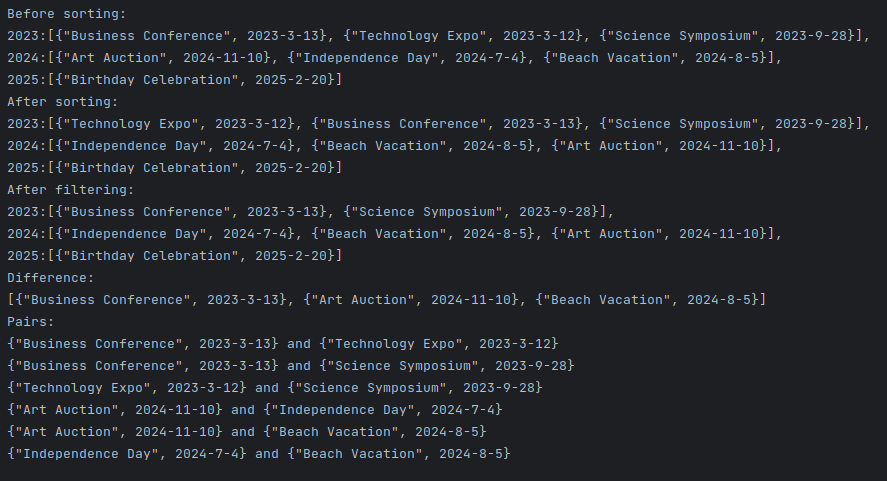
\includegraphics[scale=0.55]{1}
		\caption{Робота програми}
	\end{figure}

	\section*{Висновок}
	Під час виконання лабораторної роботи я працював з колекціями. Навчився працювати з колекціями. Визначив різницю між колекціями.
	 
\end{normalsize}
\end{document}
